\chapter{Methodology} The methodology for this project involves collecting a large and diverse dataset of sign language gestures, followed by meticulous preprocessing to normalize and annotate the data accurately. An optimized Recurrent Neural Network (RNN) model will be designed and trained to capture the temporal dynamics of these gestures, utilizing advanced machine learning techniques. The model will undergo iterative testing and validation to ensure high accuracy and efficiency, with real-time processing capabilities integrated for practical application. A user-friendly interface will be developed to ensure accessibility and ease of use across various technical proficiencies. The system will then be refined through extensive evaluation and user testing to guarantee its reliability and effectiveness in real-world scenarios.
\section{About RNN}
The methodology for developing a sign language detection system using Recurrent Neural Networks (RNNs) begins with the critical task of data collection. A comprehensive dataset of sign language videos is gathered, encompassing a diverse range of signs and expressions from multiple sign languages. This diversity is crucial for the model to generalize well across different sign languages and variations in gesture execution. The collected videos undergo rigorous preprocessing to normalize and annotate the data accurately. Frames are extracted from each video at consistent intervals, converting the raw video data into sequences of images. This step ensures that the temporal coherence necessary for effective sequence learning is maintained.

In the next phase, spatial features are extracted from these image sequences using Convolutional Neural Networks (CNNs). CNNs are highly effective in identifying and extracting significant patterns within images, making them ideal for recognizing the intricate details of sign language gestures. By converting the frames into feature vectors, CNNs transform the raw visual data into a structured format suitable for sequential processing by the RNN. These feature vectors encapsulate the critical visual information from each frame, preparing them for the temporal analysis required for accurate sign language detection.

The core of the system is the RNN model, which is specifically designed to handle and interpret sequential data. Long Short-Term Memory (LSTM) or Gated Recurrent Unit (GRU) architectures are typically employed due to their proficiency in managing long-term dependencies and retaining context over extended sequences. The RNN model is configured with input layers to accept the feature vectors produced by the CNN, hidden layers to process the temporal dynamics of these vectors, and output layers to generate predictions for the sign language labels. The hidden layers play a pivotal role as they maintain a memory of previous inputs, allowing the model to understand the sequence of gestures as a coherent flow rather than isolated events.

Training the RNN model involves a meticulous process of feeding it the annotated dataset, which is split into training, validation, and test sets. The model is trained using a loss function such as categorical cross-entropy, which quantifies the accuracy of the predictions by comparing them to the actual labels. Optimizers like Adam are used to iteratively adjust the model’s parameters to minimize the loss. Regularization techniques such as dropout are applied to prevent overfitting, ensuring that the model performs well on unseen data. This phase requires substantial computational resources and expertise in fine-tuning the model to achieve optimal performance.

To ensure the system is practical for real-world applications, it must be capable of real-time processing. The trained RNN model is employed to predict sign language labels from live image sequences captured by a camera. Temporal smoothing techniques are utilized to enhance the stability and accuracy of these real-time predictions, reducing noise and ensuring consistent output even when individual frames may be ambiguous or noisy. This real-time capability is essential for providing immediate feedback, making the system highly usable in everyday interactions.

\begin{figure}[ht]
    \centering
    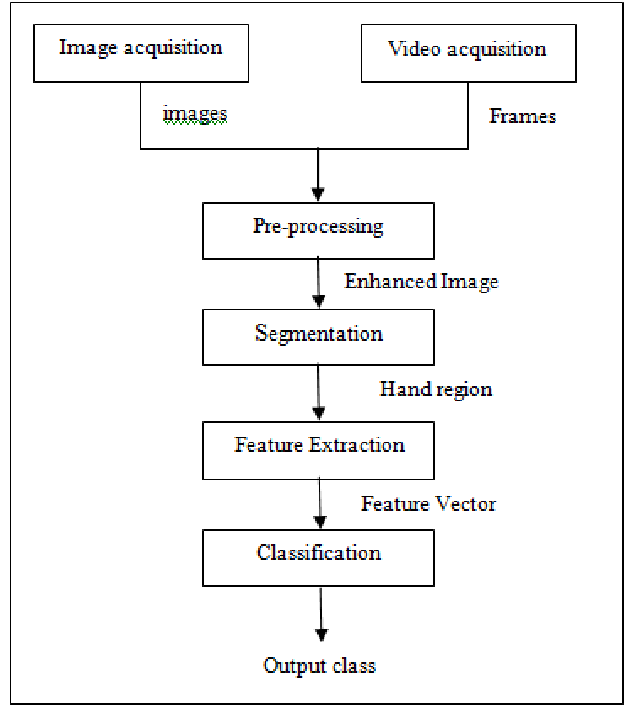
\includegraphics[width=1.0\linewidth]{images/flowchart.1.png}
\begin{figure}
        \centering
        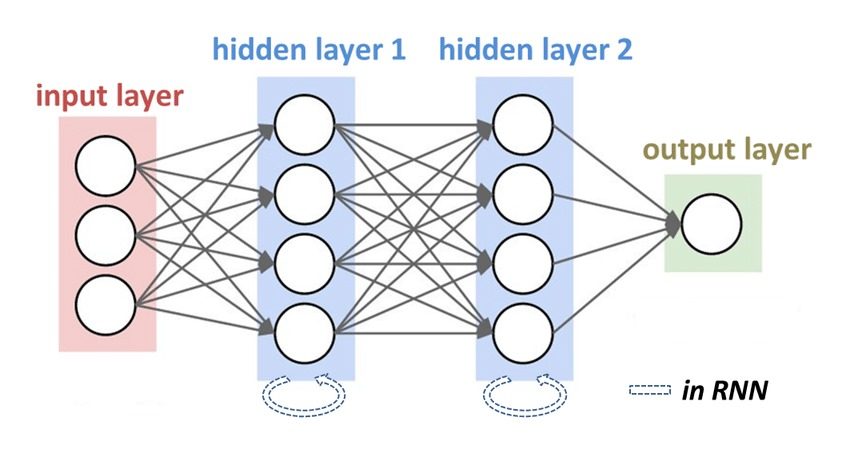
\includegraphics[width=1.0\linewidth]{images/Rnn.jpg}
        \caption{Architecture of RNN}
        \label{fig:enter-label}
    \end{figure}
        \caption{Flowchart of sign language detection}
    \label{fig:flowchart-sign-language}
\end{figure}
\newpage
\section{About  LSTM}
In this project, the Long Short-Term Memory (LSTM) algorithm will play a crucial role in accurately recognizing and interpreting sign language gestures. LSTMs are a type of recurrent neural network (RNN) architecture specifically designed to address the vanishing gradient problem, making them particularly effective for capturing long-range dependencies in sequential data. In the context of sign language detection, LSTMs will be employed to process the temporal dynamics inherent in gestures, allowing the system to effectively interpret the sequential patterns of hand movements, facial expressions, and body postures. The LSTM architecture consists of memory cells that can retain information over extended time periods, enabling the model to remember relevant context from earlier parts of the gesture sequence when making predictions. This capability is essential for accurately recognizing and distinguishing between different signs, even in complex and ambiguous scenarios. During training, the LSTM model will learn to extract meaningful features from the input sequences of image frames, adaptively adjusting its internal parameters to optimize performance. Through iterative training and validation, the LSTM will be fine-tuned to achieve high accuracy and robustness in sign language recognition. Once trained, the LSTM-based system will be capable of real-time processing, providing instantaneous translation of sign language gestures into spoken or written language, thereby enhancing accessibility and inclusivity for the deaf and hard-of-hearing community. 


\section{Flowchart}

\begin{figure}[ht]
    \centering
    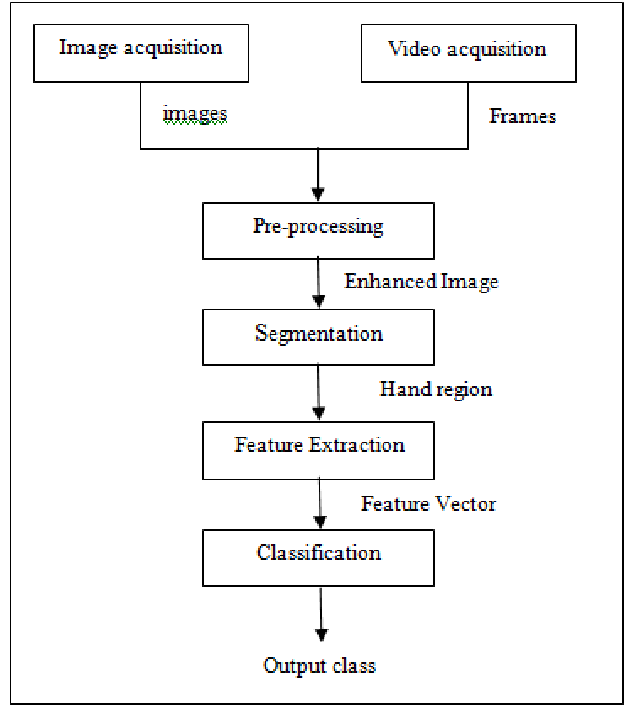
\includegraphics[width=1.0\linewidth]{images/flowchart.1.png}
    \caption{Flowchart of sign language detection}
    \label{fig:flowchart-sign-language}
\end{figure}

.